\chapter{Model Predictive Control Setup}
\label{chapter:MPC}
This chapter presents the setup and creation of the MPC controller, and investigates the performance of the resulting controller on the greenhouse environment. Moreover, the effect of the prediction horizon is investigated on both nominal and stochastic conditions. The works in this chapter is similar to what is presented in \cite{boersmaRobustSamplebasedModel2022} and \cite{morcegoReinforcementLearningModel2023}. However, direct comparisons are not possible. \cite{boersmaRobustSamplebasedModel2022} develops to create a robust sample based controller, while this chapter will focus on constructing a conventional MPC. This is done to examine the effects of uncertainty on this controller and later asses whether the integration of RL can mitigate these effects. In \cite{morcegoReinforcementLearningModel2023}, such an MPC controller is developed. However, it does not provide specific weather data. Finally the optimization goal used in this thesis differs from that in both papers. However, a qualitative comparison may be done.




\section{Greenhouse MPC problem formulation}\label{section: greenhouse MPC formulation}
In order to directly compare the performance of the MPC to RL and to the RL-MPC controller, it is important that the optimization goal is equivalent. As discussed in \autoref{ssection:optimization-goal}, it is desired to optimize the economic benefit of the greenhouse environment. Similarly to \autoref{section:env-description}, the optimization goal of the MPC is done to ensure that the sum of stage costs are equal to the actual economic benefit of the system. As such the following optimization goal is solved at every time step:

\begin{subequations} \label{eq:mpc_ocp}
	\begin{align}
		\min_{u(k),x(k)} & \sum_{k = k_0}^{k_0 + N_p-1} {l(u(k), y(k))} \\
		\text{s.t.} \quad & x(k+1) = f(x(k), u(k), d(k), p),  \label{eq:constraint-1} \\
		& y(k) = g(x(k+1), p), \label{eq:constraint-dynamics} \\
		& -\delta u_{max} \leq u(k) - u(k-1) \leq \delta u_{max}, \label{eq:constraint-delta-u} \\
		& u_{\min} \leq u(k) \leq u_{\max}, \label{eq:constraint-u-limits}\\
		& x(k_0) = x_{k_0}. \label{eq:constraint-initial}
	\end{align}
\end{subequations}

This MPC OCP is similar to what is discussed in \autoref{ssection:general-mpc}, but it does not include a terminal cost or constraint/region. Furthermore, the constraints are aligned with that of the greenhouse environment.  To ensure that the optimization goal is exactly the same as the Rl reward function (\autoref{section:env-description}), the cost function $V(u(k),y(k))$ becomes:

\begin{equation} \label{eq:mpc_stage_cost}
	\begin{aligned}
		l(u(k),y(k)) & = - c_{p_3} (y(k) - y(k-1)) + c_{p_1} u_{1} + c_{p_2} u_{2} + \sum_{i = 1}^4 s_i(k) \\
		\text{where} & \quad s_i(k) \geq 0, \\
		& s_1(k) \geq c_{p_{C02}} \cdot (y_2^{min} - y_2(k)), \\ 
		& s_2(k) \geq c_{p_{C02}} \cdot (y_2(k) + y_2^{max}), \\ 
		& s_3(k) \geq c_{p_{T_{lb}}} \cdot (y_3^{min} - y_3(k)), \\ 
		& s_4(k) \geq c_{p_{T_{ub}}} \cdot (y_3(k) + y_3^{max}), \\ 
		& s_5(k) \geq c_{p_{H}} \cdot (y_4^{min} - y_4(k)), \\ 
		& s_6(k) \geq c_{p_{H}} \cdot (y_4(k) + y_4^{max}), \\
	\end{aligned}	
\end{equation}

where the slack variables are introduced in order to accommodate the output constraint in equation \autoref{eq:mpc_ocp}, resulting in an optimization problem equivalent to that of RL. The penalty constants $c_{p_{C02}},c_{p_{T_{lb}}},c_{p_{T_{ub}}},c_{p_{H}}$ are the same as what is used in the Rl problem formulation and given in \autoref{tab:pen-constants}. While MPC can impose hard constraints on the states of the system, and is one of its advantages over RL, it was decided that for a direct comparison between algorithms, the same constraints must be given. Lastly, the policy generated by the MPC is denoted $\kappa(x,u,d,p)$ where the optimal control action to take at time k $k$ is

\begin{equation}\label{eq:mpc_policy_notation}
	u_k^* = \kappa(x_k,u_{k-1}^*, d_k, p)
\end{equation}

\paragraph{Experimental Setup} Furthermore, the experimental setup is identical to what is used in \autoref{section:experimental-setup} with the exception of normalizing observations. The performance metrics are the sum of the stage costs during the simulation period, which is equivalent to the EPI minus the sum of the state violations. For the stochastic environment, the performance metric is calculated by taking the average of the sum of stage costs over 30 simulation periods, as well as considering the variance of the resulting stage costs. In the case of stochasticity, the MPC algorithm still solves the optimization problem defined by equation \autoref{eq:mpc_ocp} using the nominal system parameters. However, it is only during the system evolution that the uncertainty in parameters is taken into account. 

Finally, to increase the computational time and feasibility of the MPC solver, the solver is warm-started with the previous solution to reduce the number of iterations required to reach the optimal solution  \footnote{The solution to the OCP is heavily reliant on initial guesses due to the non-linearity nature of the problem, lagrangian multipliers from the previous solutions were also reused to mitigate instability in the solver. These instabilities are especially prevalent in longer prediction horizons}. The computational time of computing the optimal control actions will also be examined for each prediction horizon. These performance metrics are given for all prediction horizons. Finally, The MPC framework is built using the open source software Casadi \cite{Andersson2018} and the non-linear solver IPOPT \cite{wachterImplementationInteriorpointFilter2006} in python. 

\section{Deterministic Results}
Simulations are conducted for every prediction horizon $N_p$.The prediction horizons to be tested will include time intervals of 1 hour, 2 hours, 3 hours, 4 hours, 5 hours, and 6 hours. Results include the final cumulative reward and the average time required to solve \autoref{eq:mpc_ocp} for each prediction horizon (averaged across the growing period).

\begin{figure}[H]
	\centering
	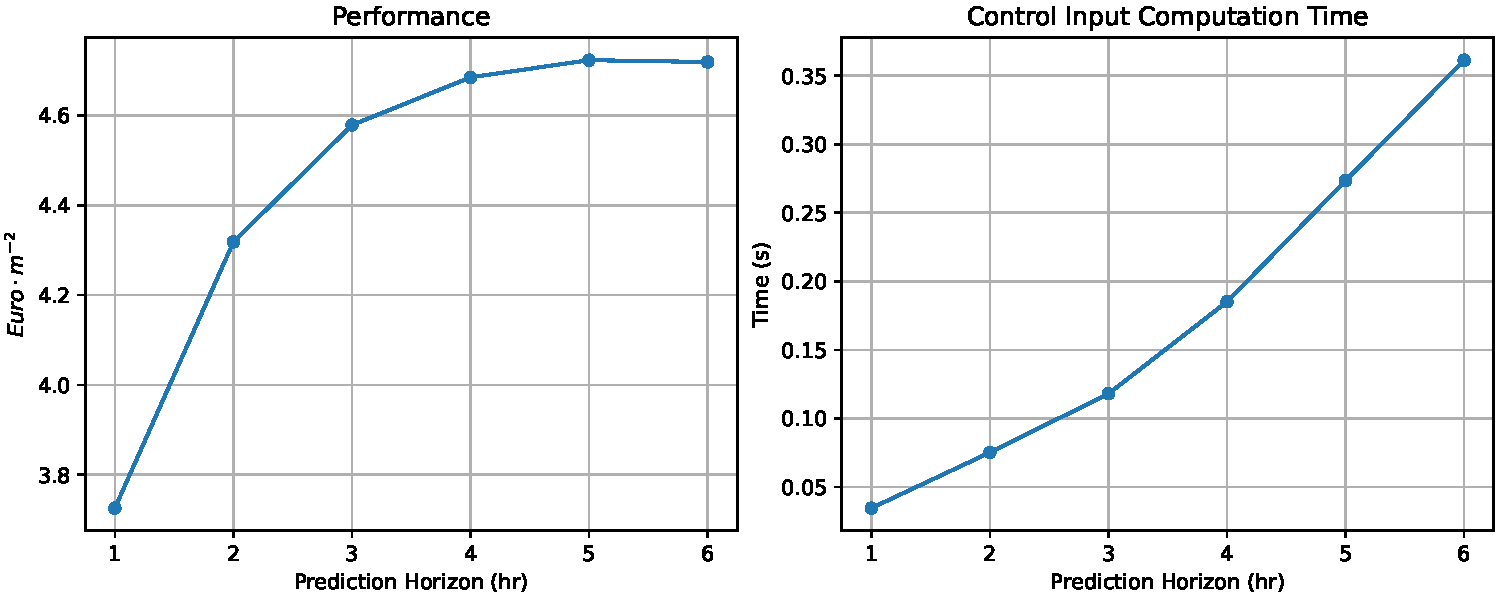
\includegraphics[width=\textwidth]{figures/mpc_nominal.pdf}
	\caption{The final cumulative reward achieved using nominal MPC and the average computation time for each prediction horizon}
	\label{fig:nominal_mpc_perf}
\end{figure}

\autoref{fig:nominal_mpc_perf} exhibits the performance and the computational time of the MPC for each prediction horizon respectively. It it can be seen that performance increases with an increase in prediction horizon up until 6 hrs. This increase in performance however is not guaranteed for an economic model predictive controller as stated in \cite{ellisTutorialReviewEconomic2014}  and \cite{amritEconomicOptimizationUsing2011}, without a sufficiently long time horizon or an appropriate terminal cost function or constraints. Although not entirely clear in \autoref{fig:nominal_mpc_perf}, a prediction horizon of 6hr, actually produces a slightly lower performing policy than with a prediction horizon of 5 hours. Whether this is due to instabilities in the solver or the nature of the economic optimization problem remains uncertain. \\
As expected, the computational time in computing the control action increases with an increase in complexity. It is noted that the RL algorithm is able to calculate the control action in approximately 0.2 milliseconds, while the fastest MPC controller, with a prediction horizon of 1 hour, takes approximately 35 milliseconds, making it nearly 175 times slower.  While this outcome is not surprising, it effectively demonstrates the computational demand of MPC, specifically for a highly non-linear model. Nevertheless, the process of setting up and implementing the MPC controller was considerably easier compared to RL. RL, on the other hand, demanded extensive time investment in fine-tuning hyperparameters. Despite all the fine-tuning in RL, MPC still outperforms the RL agent, this performance difference is analyzed in \autoref{chapter:deterministic_RL_MPC}. 

\begin{figure}[H]
	\centering
	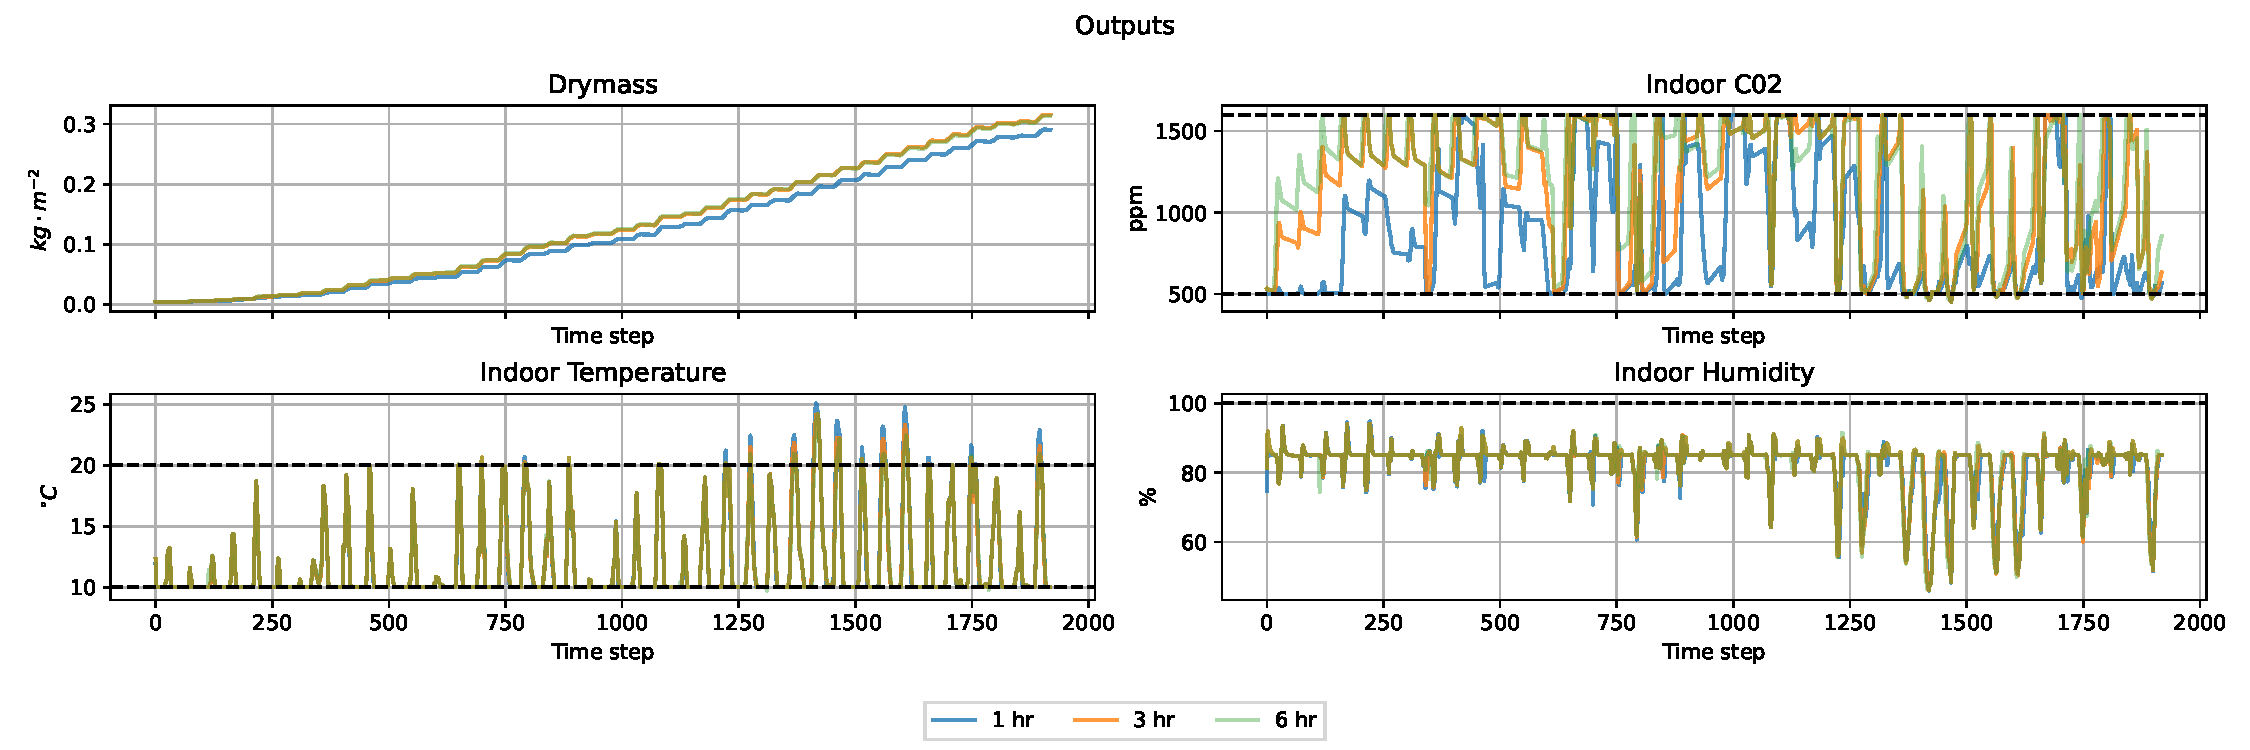
\includegraphics[width=\textwidth]{figures/mpc_outputs_time_series.pdf}
	\caption{MPC 1hr and 5hr Time series of greenhouse outputs}
	\label{fig:mpc-timeseries-outputs}
\end{figure}

\begin{figure}[H]
	\centering
	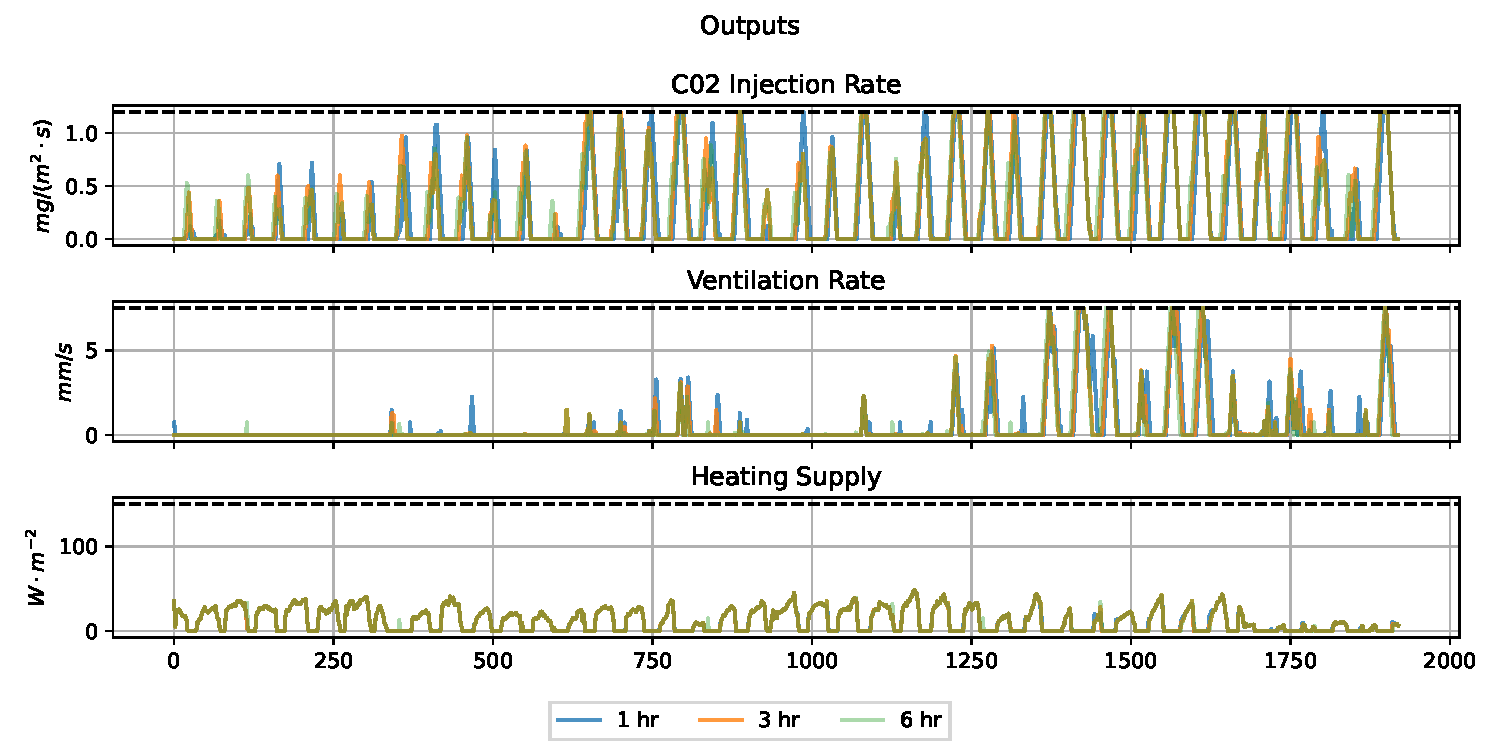
\includegraphics[width=\textwidth]{figures/mpc_inputs_times_series.pdf}
	\caption{MPC 1hr and 5hr time series of controller inputs}
	\label{fig:mpc-timeseries-inputs}
\end{figure}

\autoref{fig:mpc-timeseries-outputs} and \autoref{fig:mpc-timeseries-inputs} displays the trajectories of the states and inputs of the best performing MPC controller (5hr prediction horizon) and the worst performing (1 hr). These bear similarities to those of the RL agents \autoref{fig:selected-policies-outputs} and \autoref{fig:selected-policies-inputs} respectively. It is noted that in both cases (RL and MPC), the better performing policies rapidly raises the indoor C02 levels at the beginning of the growing period by reducing ventilation and increasing C02 injection. However, the trajectories of other states and inputs, particularly the indoor temperature, humidity and heating, appear to be unchanged. Either the temperature does not play a vital role in plant growth or the prediction horizon is not long enough to see the effect of temperature at initial growth stages. However, it is clear that the MPC controller uses heating at night and the irradiance during the day to ensure that temperature constraints are met. These results are very similar to \cite{morcegoReinforcementLearningModel2023} and \cite{boersmaRobustSamplebasedModel2022} although difficult to compare quantitatively due to the difference in the optimization goal and MPC problem formulation.


\section{Stochastic Results}
For each stochastic level, $\delta = 5\%, \delta = 10\%, \delta = 20\%$, was analyzed with prediction horizons of 1, 3, and 5 hours. Additional prediction horizons were not considered due to limitations in simulation time. 

\begin{figure}[H]
	\centering
	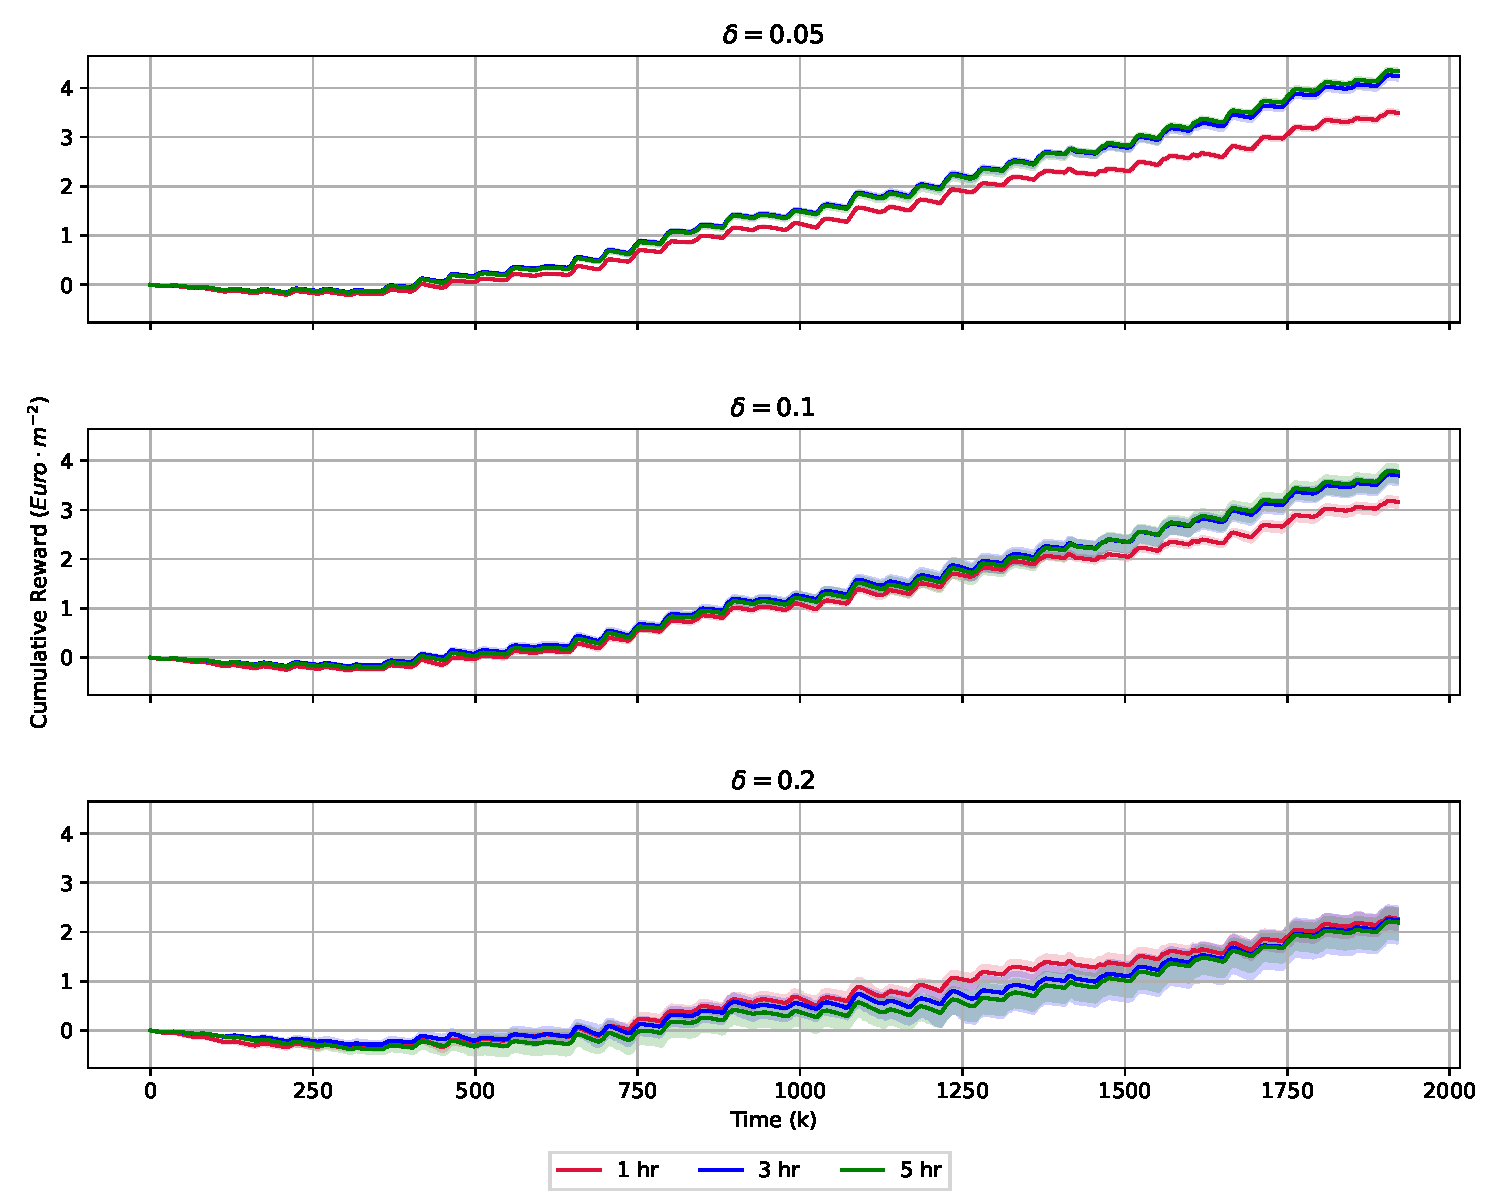
\includegraphics[width=0.8\textwidth]{figures/stochastic_mpc_rewards_time.pdf}
	\caption{Time evolution of cumulative Rewards. Displays the evolution of the cumulative reward over the growing period, for each level of stochastic and prediction horizon. Solid lines represent the mean cumulative reward trajectory with a range indicating the minimum and maximum trajectory recorded in the 30 runs.}
	\label{fig:stochastic-mpc-rewards-time}
\end{figure}

\autoref{fig:stochastic-mpc-rewards-time} shows the impact of introducing uncertainty and its effect on the cumulative reward obtained by the MPC controller at each time step. While a $\delta = 0.05$ does not noticeable impact performance, there is significant performance degradation for $\delta = 0.2$. Also to note, is that a longer prediction still results in a higher mean cumulative reward, however for high uncertainties, specifically $\delta = 0.2$, it seems that a longer prediction horizon might not result in the desired performance increase.

\begin{figure}[H]
	\centering
	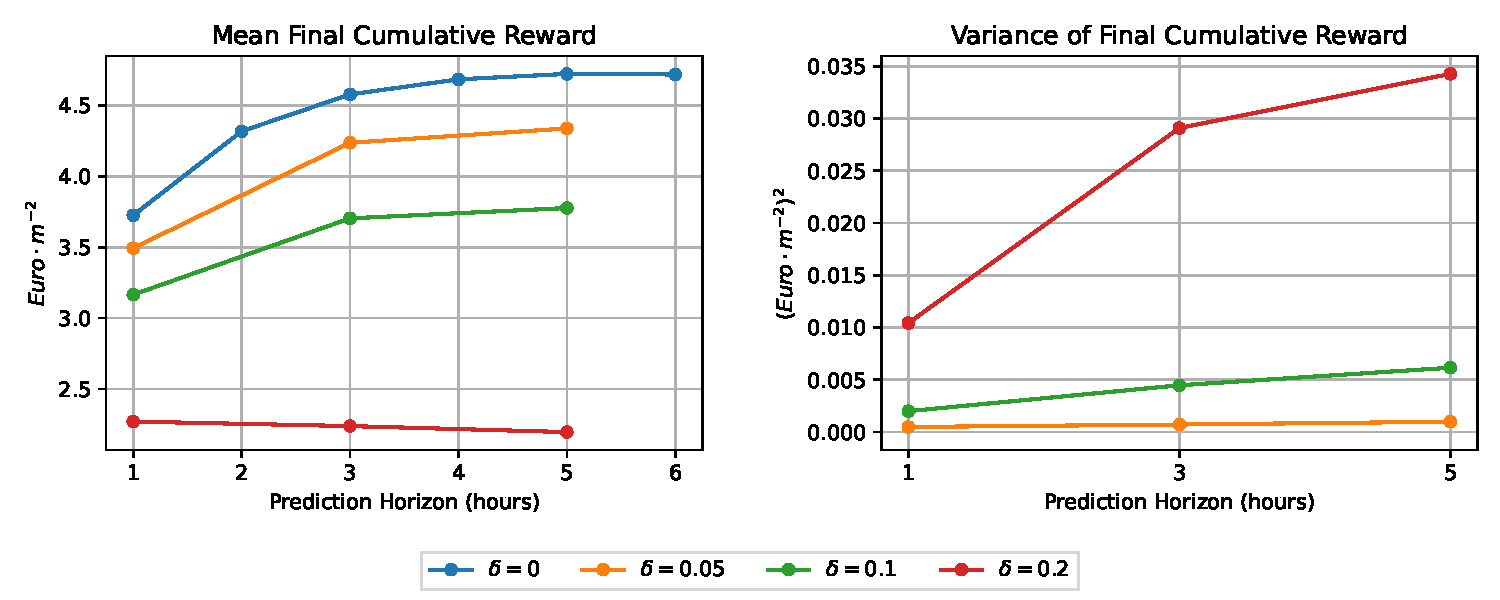
\includegraphics[width=\textwidth]{figures/stochastic_mpc_perf.pdf}
	\caption{MPC performance in stochastic conditions }
	\label{fig:stochastic-mpc-perf}
\end{figure}

\autoref{fig:stochastic-mpc-perf} depicts the final mean and variance values of the cumulative reward for each prediction horizon and uncertainty level, including nominal conditions. \autoref{fig:stochastic-mpc-perf} may provide a better representation of how stochasticity affects the final performance. Longer prediction horizons appear to have less performance increases and might become detrimental at very high uncertainty levels. Moreover, there is a clear adverse affect on variance as prediction horizon is increased for all uncertainty levels. This can be attributed to the fact that longer prediction horizons become progressively less accurate due to the increasing uncertainty of the model parameters. It is widely acknowledged that a conventional MPC is not adept at handling uncertainty (although methods such as state estimation exists), and these results are confirmation of this. Although it is possible to formulate a robust MPC, such as in \cite{boersmaRobustSamplebasedModel2022}, it introduces a heavy computational burden on the controller. As previously mentioned, RL's decrease in performance due to uncertainty is not as drastic as MPC's. Thus, it is worth exploring whether the RL agent can assist the MPC in mitigating the adverse impacts of parametric uncertainty.


\section{Conclusion}
In conclusion, this chapter has presented the setup and implementation of the MPC framework whereby the EMPC OCP was designed to maximise the economic advantage of the greenhouse by aligning its optimisation objective with the optimisation goal specified in \autoref{ssection:optimization-goal}. However, additional slack variables were introduced to align the optimisation problem with what the RL agent is optimising for more meaningful comparisons. The MPC controller's performance was thoroughly examined under both nominal and stochastic conditions, focusing on various prediction horizons. The findings and comparisons drawn in this chapter shed light on the controller's efficacy and limitations in managing a greenhouse environment.

Under deterministic conditions, MPC exhibited varying performance across different prediction horizons.. It demonstrated improved economic outcomes with longer prediction horizons, albeit with increased computational demands. However increasing the prediction horizon does not gaurentee an increase in performance without an adequate terminal cost function and/or terminal constraint/region. Notably, while MPC RL in performance under deterministic settings, its computational overhead was significantly higher, highlighting a trade-off between computational efficiency and performance optimization. The scalability of the computational time is considerably inferior to that of the RL agent. Therefore in more complex systems, the model is typically linearized or simplified, leading to a suboptimal policy.

Furthermore, stochastic simulations revealed MPC's vulnerability to uncertainty in the environment. Increasing uncertainty levels adversely affected MPC's performance, whereby increasing the prediction horizon may become harmful under extreme uncertainty , leading to compromised economic benefits and increased variability in the final cumulative reward. These results underscored MPC's limited robustness against stochastic influences compared to RL approaches.

In conclusion, while MPC proved effective in deterministic scenarios with appropriate prediction horizons, its performance degradation under stochastic conditions necessitates exploration of hybrid RL-MPC strategies to enhance its performance and robustness. To guarantee performance for an EMPC, appropriate additions to its formulation must be made, which the RL agent could potentially solve.

